\documentclass{beamer}

%% \usetheme{Warsaw}
\usetheme{EastLansing}
%% \usecolortheme{beetle}

\title[Functional Programming]{An Introduction to Functional Programming}
\author{Andreas Pauley -- @apauley}
\institute{Pattern Matched Technologies\\Lambda Luminaries @lambdaluminary}
\date{September 2, 2013}

\usepackage[utf8]{inputenc}
\usepackage{graphicx}
\usepackage{listings}
\usepackage{minted}

\usepackage{hyperref}

\AtBeginSection[]
{
  \begin{frame}
    \frametitle{Table of Contents}
    \tableofcontents[currentsection]
  \end{frame}
}

\begin{document}

\lstset{
  basicstyle=\ttfamily\bfseries,
  commentstyle=\color{red}\itshape,
  stringstyle=\color{green},
  showstringspaces=false,
  numbers=left,
  keywordstyle=\color{blue}\bfseries}

\begin{frame}
  \titlepage
\end{frame}

\begin{frame}{Pattern Matched Technologies}
  
\includegraphics[scale=0.21]{img/pmt-logo.png}

  Developing financial applications in Erlang.

  \url{http://www.patternmatched.com/}
\end{frame}

\begin{frame}{Lambda Luminaries -- @lambdaluminary}
  \framesubtitle{Local functional programming user group}
  We meet once a month, on the second Monday of the month.

  \url{http://www.meetup.com/lambda-luminaries/}
  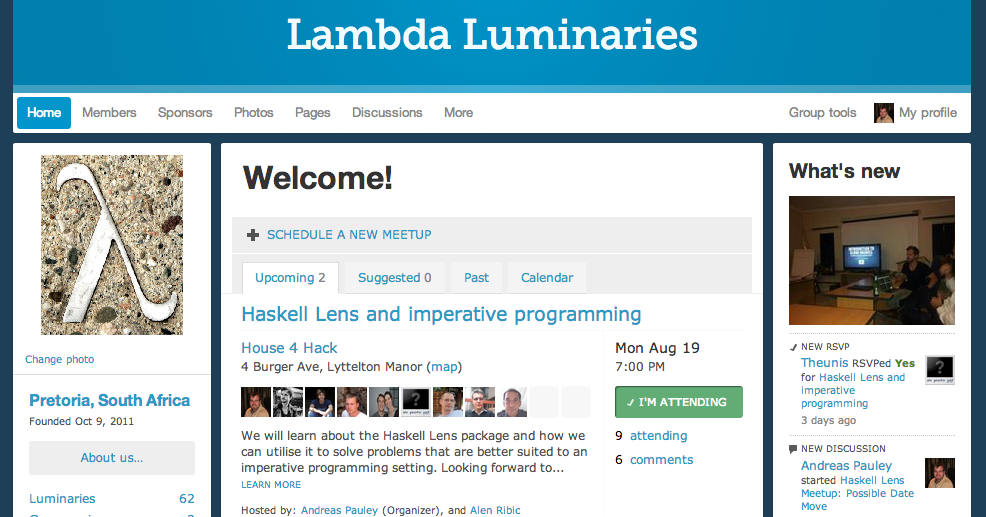
\includegraphics[scale=0.3]{img/LambdaLuminariesScreenShot2013-08-09.png}
\end{frame}

\section{Introduction}

\begin{frame}{A word from the wise}
  \begin{exampleblock}{}
    {\Large ``
      No matter what language you work in, programming
      in a functional style provides benefits.
      You should do it whenever it is convenient, and you
      should think hard about the decision when it isn’t convenient.
      ''}
    \vskip5mm
    \hspace*\fill{\small--- John Carmack, ID Software \cite{carmack}}
  \end{exampleblock}
\end{frame}

\begin{frame}{Quake}
  
\includegraphics[scale=0.4]{img/quake.png}
\end{frame}


\begin{frame}{A Few Functional Programming Languages}

  \begin{description}[<+->]
  \item [Haskell] Strong focus on functional purity. Lazy evaluation.
    Advanced static type system. Native-code compiler.
  \item [Erlang] Focused around concurrency and distributed
    programming. Strict evaluation. Dynamic typing. Runs on the BEAM VM.
  \item [Clojure] A modern Lisp language. Focus on concurrency. Lazy
    evaluation. Dynamic typing. Runs on the JVM.
  \item [Scala] FP and OO. Strict evaluation by default,
    but supports lazy evaluation. Advanced static type system. Runs on the JVM.
  \item [F\#] FP and OO. Strict evaluation by default,
    but supports lazy evaluation. Advanced static type system. Runs on
    the .NET CLR.
  \item [OCaml] Part of the ML family. Sometimes claimed to be ``faster
    than C''. Strict evaluation. Advanced static type system. Native-code compiler.
  \end{description}

\end{frame}

\section{Definition of Functional Programming (attempt \#1)}

\begin{frame}{}
  So what exactly is Functional Programming?
\end{frame}

\begin{frame}{Functional Programming, noun:}

  \begin{exampleblock}{}
    {\Huge ``
      Functional Programming is a list of things you CAN’T do.
      ''}
    \vskip5mm
    \hspace*\fill{\small \cite{pauleyfp}}
  \end{exampleblock}
\end{frame}

\begin{frame}
  When programming in a functional style/language:
  \begin{itemize}[<+->]
  \item You can't vary your variables.
  \item You can't mutate or change your state.
  \item No while/for loops, sorry.
  \item You can't have side-effects.
  \item You can't control the order of execution (lazy evaluated languages).
  \end{itemize}
\end{frame}

\begin{frame}{Are you kidding me?}
  How can anyone program like this???
  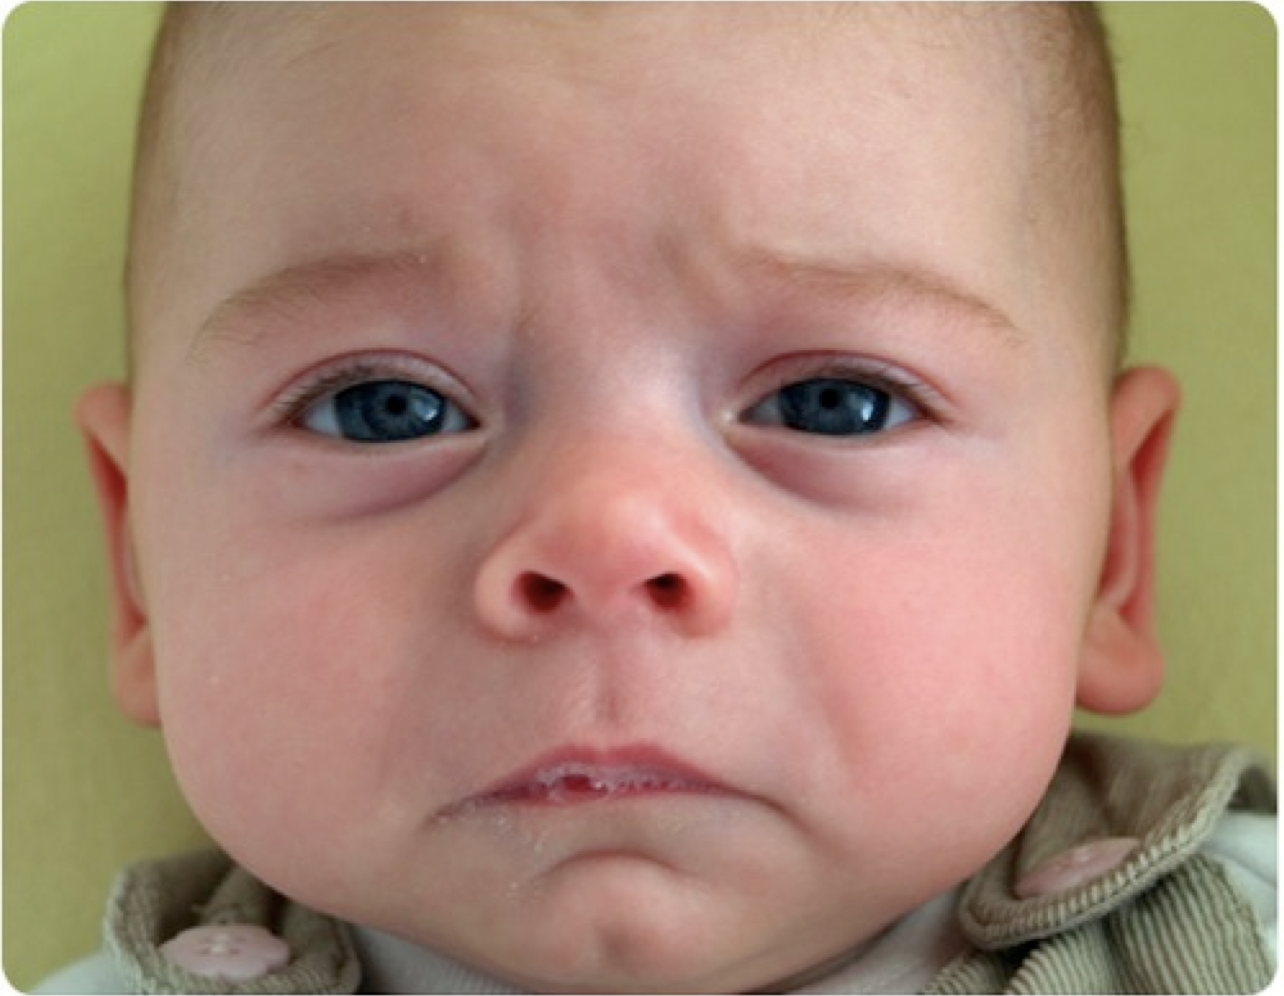
\includegraphics[scale=0.3]{img/sadbaby.png}
\end{frame}

\begin{frame}{GOTO 10}
    This sounds like
  \begin{exampleblock}{}
    {\Large ``You can't have GOTO statements''}
  \end{exampleblock}
  \vskip5mm
  \hspace*\fill{\small See Hughes and Dijkstra \cite{whyfp, dijkstra}}

  \begin{itemize}[<+->]
  \item Also framed in the negative (you can't).
  \item In hindsight we don't really need GOTO's.
  \item In hindsight it is not about what you cannot do.
  \end{itemize}
\end{frame}

\begin{frame}{Structured Programming and Functional Programming}
  \begin{description}[<+->]
  \item[Structured Programming] introduced subroutines with fixed
    entry/exit points (instead of GOTO's), resulting in improved
    modularity.
  \item[Functional Programming] provides similar important benefits --
    more about this later.
  \end{description}
\end{frame}

\begin{frame}{}

  {\Large We need a better definition for Functional Programming.}

\end{frame}

\section{Definition of Functional Programming (attempt \#2)}

\begin{frame}{Functional Programming, noun:}

\begin{exampleblock}{}
  {\Large ``
  Functional programming is so called because a program consists entirely of functions.
  ''}
  \vskip5mm
  \hspace*\fill{\small--- John Hughes, Why Functional Programming
    Matters \cite[p.~1]{whyfp}}
\end{exampleblock}
\end{frame}

\section{Function Recap}

\begin{frame}{}
OK... so what exactly is a function?
\end{frame}

\begin{frame}{An example function}

  {\Huge $f(x) = 2x + 3$}

\end{frame}

\begin{frame}{Variables in functions}

  {\Huge $f(x) = 2x + 3$}

When we evaluate the function:
  \begin{itemize}[<+->]
    \item $f(4) = 2*4 + 3 = 11$
    \item The value of $x$ will not change inside the function body.
    \item No $x = 4$ and later $x = 21$ in the same function body.
    \item Same input, same output. Every time.
    \item In other words, we can replace any occurrence of $f(4)$ with
      $11$ (Referential Transparency)
  \end{itemize}
\end{frame}


\begin{frame}{Functions can call other functions}

  {\Huge $g(x) = f(x) + 1$}

\end{frame}

\begin{frame}{Values are functions}

  {\large Constant values are just functions with no input parameters}
  \\
  {\Huge $k = 42$}

\end{frame}

\begin{frame}{Functions can be combined}

  {\Huge $h(x) = f(g(x))$}

\end{frame}

\begin{frame}{Higher-order Functions}

  {\Large Functions can take functions as input and/or return
    functions as the result.}

  \begin{itemize}[<+->]
  \item {\Huge $h(p, q, x) = p(x) + q(2)$}
  \item {\Huge $h(f, g, 3) = f(3) + g(2)$}
  \end{itemize}

\end{frame}

\begin{frame}{A functional program consists entirely of functions}

  \inputminted[firstline=3]{python}{code/justfunctions.py}

\end{frame}

\begin{frame}{A functional program consists entirely of functions}

  \inputminted{haskell}{code/justfunctions.hs}

\end{frame}

\section{Object-Oriented Programming and Functional Programming}

\begin{frame}

  \begin{exampleblock}{}
    {\Large ``
      OO makes code understandable by encapsulating
      moving parts.
      FP makes code understandable by minimizing moving
      parts.
      ''}
    \vskip5mm
    \hspace*\fill{\small--- Michael Feathers, @mfeathers \cite{mfeathers}}
  \end{exampleblock}

\end{frame}

\begin{frame}{Overlap between FP and OO}

  {\Large Both OO and FP share a lot of the same
    concerns.}

  \begin{itemize}[<+->]
  \item {\Large How can we best write stable and bug-free programs?}
  \item {\Large How can we best write maintainable code?}
  \item {\Large What are the basic building blocks of our software?}
  \item {\Large How can we combine these building blocks to build big
    systems?}
  \end{itemize}

\end{frame}


\begin{frame}{Overlap between FP and OO}

  {\Large Some principles that are valued by both Object-Oriented
    Programming and Functional Programming:}

  \begin{itemize}[<+->]
  \item DRY (Don't Repeat Yourself)
  \item Separation of Concerns
  \item High Cohesion, Low Coupling
  \end{itemize}

\end{frame}

\begin{frame}{High Cohesion, Low Coupling}

  \begin{description}[<+->]
  \item[High Cohesion] Related concepts are grouped together.
  \item[Low Coupling] Changes in one part of a program does not
    affect other parts.
  \end{description}
\end{frame}

\begin{frame}{A thought experiment}

  {\Huge What happens if we take low coupling to the extreme?}

\end{frame}

\begin{frame}[fragile]{Coupling in OO and FP}

  \begin{description}[<+->]
  \item[OO] An object couples state (data) and behaviour.
    \begin{lstlisting}
      person.age()
    \end{lstlisting}
  \item[FP] Functions define behaviour. State is decoupled, typically
    passed as parameters to functions.
    \begin{lstlisting}
      age(person)
    \end{lstlisting}
  \end{description}

\end{frame}

\section{Common FP Idioms}
\subsection{Recursion}

\begin{frame}[fragile]{Recursive function: Haskell}

Haskell function definition:
  \lstinputlisting[language=Haskell, firstline=3,lastline=5]{code/doubleall_recursion.hs}

Example use in the interactive interpreter:
  \begin{lstlisting}[language=Haskell]
Prelude Main> doubleAll [8,2,3]
[16,4,6]
  \end{lstlisting}

\end{frame}

\begin{frame}[fragile]{Recursive function: Python}

Function definition:
  \lstinputlisting[language=Python, firstline=3]{code/doubleall_recursion.py}

Example use in the interactive interpreter:
  \begin{lstlisting}[language=Python]
>>> doubleAll([8,2,3])
[16, 4, 6]
  \end{lstlisting}

\end{frame}

\begin{frame}{An iterative version in Python}

Function definition:
  \lstinputlisting[language=Python, firstline=3]{code/doubleall_iterative.py}
\end{frame}

\subsection{Pattern Matching}

\begin{frame}{Pattern Matching: Haskell}

  \lstinputlisting[language=Haskell, firstline=3,lastline=5]{code/doubleall_recursion.hs}

\end{frame}

\subsection{Higher-order Functions}

\begin{frame}{Higher-order functions: Python}

  \lstinputlisting[language=Python, firstline=3,lastline=10]{code/higher_order.py}

\end{frame}

\begin{frame}{Higher-order functions: Haskell}

  \lstinputlisting[language=Haskell, firstline=3,lastline=8]{code/higher_order.hs}

\end{frame}


\subsection{List Comprehensions}

\begin{frame}[fragile]{List Comprehensions}

Python:
  \begin{lstlisting}[language=Python]
>>> [x*2 for x in range(1,6)]
[2, 4, 6, 8, 10]
  \end{lstlisting}

Haskell:
  \begin{lstlisting}[language=Haskell]
Prelude> [x*2 | x <- [1..5]]
[2,4,6,8,10]
  \end{lstlisting}

\end{frame}

\section{Higher-order Functions and Lists}

\begin{frame}{3 Basic List Operations}

  \begin{description}[<+->]
  \item[Map] Convert each element of a list into some other value.
    Example: Convert a list of students to a list of phone numbers.
  \item[Filter] Get a subset of a list based on some condition.
    Example: Filter the entire list of students down to only those
    that passed the exam.
  \item[Fold] Reduce a list of items to a single value.
    Example: Reduce the list of exam percentages to the average percentage.
  \end{description}

\end{frame}

\section{Advantages of Functional Programming}

\begin{frame}{Perlisism \#19}

\begin{exampleblock}{}
  {\Large ``
    A language that doesn't affect the way you think about programming, is not worth knowing.
  ''}
  \vskip5mm
  \hspace*\fill{\small--- Alan Perlis\cite{perlis19}}
\end{exampleblock}

\end{frame}

\begin{frame}{Advantages of Functional Programming}

  \begin{itemize}[<+->]
  \item Changes the way you think about programming and problem solving.
  \item Improvements on the types of abstractions we can do with eg.
    higher-order functions.
  \item Lock-free concurrency.
  \item Improved ways of testing - QuickCheck.
  \item Type system does not accept Null values. Goodbye NullPointerException.
  \end{itemize}

\end{frame}

\section{Disdvantages of Functional Programming}

\begin{frame}{Disadvantages of Functional Programming}

  \begin{itemize}[<+->]
  \item Steep learning curve.
  \item There are some very cryptic concepts.
  \item Tools/IDE's are not as advanced as the mainstream equivalents.
  \item Order of execution may be difficult to reason about in a lazy language.
  \end{itemize}

\end{frame}


\begin{frame}{Unfamiliar Territory}

  {\Large Functional Programming is unfamiliar territory for most.}

\begin{exampleblock}{}
  {\Large ``
    If you want everything to be familiar you will never learn anything new.
  ''}
  \vskip5mm
  \hspace*\fill{\small--- Rich Hickey, author of Clojure\cite{hickey}}
\end{exampleblock}

\end{frame}

\section{Companies using Functional Programming}

\begin{frame}[allowframebreaks]{Companies In South Africa}

  \begin{description}[<+->]
  \item[Pattern Matched Technologies, Midrand] Using Erlang for all systems,
    eg. processing high volumes of financial transactions.
  \item[Rheo Systems, Pretoria] Using Clojure for supply chain integration.
  \item[Eldo Energy, Johannesburg] Using Clojure for intelligent monitoring of consumer
    energy.
  \item[Effective Control Systems, Kyalami] Using Erlang for print
    management.
  \item[Mira Networks, Somerset West] Using Erlang for billing
    administration and mobile development.
  \item[Amazon.com, Cape Town] Using Scala in EC2.
  \end{description}

\end{frame}

\section{References}

\begin{frame}[allowframebreaks]{References}
  \begin{thebibliography}{10}
    \bibitem{whyfp}
      John Hughes
      \newblock Why Functional Programming Matters
      \newblock \url{http://www.cs.kent.ac.uk/people/staff/dat/miranda/whyfp90.pdf}
    \bibitem{carmack}
      John Carmack
      \newblock Functional Programming in C++
      \newblock \url{http://www.altdevblogaday.com/2012/04/26/functional-programming-in-c/}
    \bibitem{dijkstra}
      Edsger W. Dijkstra
      \newblock Go To Statement Considered Harmful
      \newblock \url{http://www.u.arizona.edu/~rubinson/copyright_violations/Go_To_Considered_Harmful.html}
    \bibitem{mfeathers}
      Tweet by Michael Feathers
      \newblock \url{https://twitter.com/mfeathers/status/29581296216}
    \bibitem{perlis19}
      Alan Jay Perlis
      \newblock \url{http://www.cs.yale.edu/quotes.html}
    \bibitem{hickey}
      Rich Hickey
      \newblock \url{http://www.infoq.com/presentations/Simple-Made-Easy}
    \bibitem{pauleyfp}
      Andreas Pauley
      \newblock An Introduction to Functional Programming
      \newblock \url{https://github.com/apauley/fp_presentation}
  \end{thebibliography}
\end{frame}

\end{document}
